\section{Results II: the strengthened pipeline against the leaderboard (Amendment 2)}
\label{sec:results2}

\subsection{Primary endpoint: final pipeline versus the board leader}
Table~\ref{tab:a2leader} compares the frozen Amendment-2 pipeline with the leader of each per-task leaderboard. The comparison is paired over the same official test compositions, using the leaders' public predictions.

\textbf{expt\_gap.} The final pipeline reached an MAE of \AtwoFinalGap{}~eV against \AtwoLeaderGap{}~eV for Darwin, a fine-tuned large language model and the current leader ($\Delta=\AtwoDeltaGap$~eV, 95\% CI [\AtwoCIloGap, \AtwoCIhiGap], \AtwoPHolmExprGap). This is the only task where the pre-registered rule for ``beats the leader'' is met. It would place first among the \AtwoNEntriesGap{} entries.

\textbf{expt\_is\_metal.} The balanced accuracy of \AtwoFinalMetal{} is on par with Darwin's \AtwoLeaderMetal{} (\AtwoPHolmExprMetal). It would rank \AtwoRankMetal{} of \AtwoNEntriesMetal.

\textbf{steels.} The MAE of \AtwoFinalSteels{}~MPa is on par with TPOT-Mat's \AtwoLeaderSteels{}~MPa (95\% CI [\AtwoCIloSteels, \AtwoCIhiSteels]~MPa, \AtwoPHolmExprSteels). It would rank \AtwoRankSteels{} of \AtwoNEntriesSteels.

\textbf{glass.} The pipeline remains clearly behind MODNet v0.1.12: balanced accuracy \AtwoFinalGlass{} versus \AtwoLeaderGlass{}, \AtwoPHolmExprGlass. MODNet's probabilities, which are available in its submission, also give a much higher probability ROC-AUC (\AtwoLeaderAUCGlass{} versus our \AtwoAUCGlass).

\begin{table}[t]
\centering
\caption{Amendment-2 final pipeline versus the leaderboard leader of each task. The comparison is paired over the same official test compositions, using the leaders' public per-sample predictions. Metric semantics follow the board: MAE; balanced accuracy for classification (ours at the inner-CV threshold; Darwin's recorded labels; MODNet's probabilities at 0.5, as the board scored them). $\Delta$ is ours minus the leader. CI: paired bootstrap over test points within folds ($B=10^4$). Holm correction over four tasks. Rank: among the board entries of 18 October 2026, including ours.}
\label{tab:a2leader}
\begin{adjustbox}{max width=\textwidth}
\begin{tabular}{llccccc}
\toprule
Task & Metric & Final pipeline & Leader (board) & $\Delta$ [95\% CI] & $p_\mathrm{Holm}$ & Rank \\
\midrule
steels & MAE & 80.10 $\pm$ 10.19 & TPOT-Mat: 79.95 & +0.1577 [-4.54, +4.89] & 0.928 & 2 of 12 \\
expt\_gap & MAE & 0.2352 $\pm$ 0.0167 & Darwin: 0.2865 & -0.05131 [-0.0701, -0.0331] & $<$0.001 & 1 of 13 \\
expt\_is\_metal & bal.\ acc. & 0.9547 $\pm$ 0.0033 & Darwin: 0.9598 & -0.005093 [-0.0118, +0.00179] & 0.299 & 2 of 8 \\
glass & bal.\ acc. & 0.8937 $\pm$ 0.0158 & MODNet (v0.1.12): 0.9603 & -0.06658 [-0.0759, -0.0573] & $<$0.001 & 2 of 8 \\
\bottomrule
\end{tabular}

\end{adjustbox}
\end{table}

\begin{figure}[t]
\centering
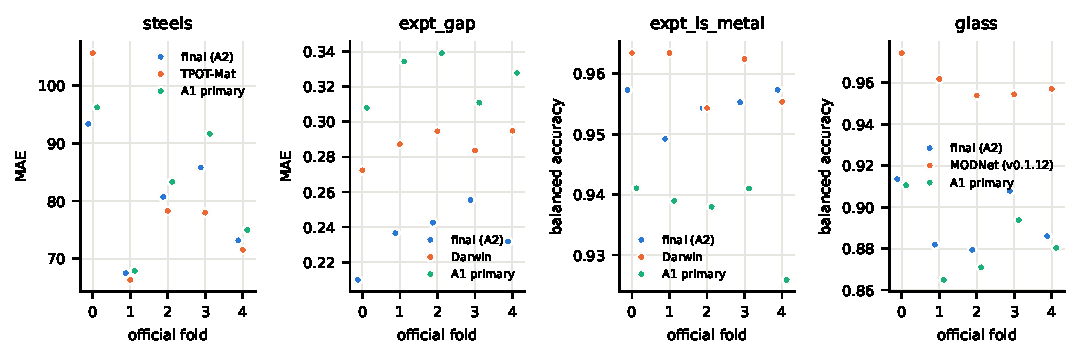
\includegraphics[width=\textwidth]{figures/fig_a2_leader.pdf}
\caption{Per-fold board metric of the Amendment-2 final pipeline, the task leader and the Amendment-1 primary arm.}
\label{fig:a2}
\end{figure}

\subsection{What changed between the two pre-registered runs}
Table~\ref{tab:a1a2} compares the two frozen pipelines on the board metric.
The largest gain is on expt\_gap, where the MAE fell from \AoneBoardGap{} to \AtwoFinalGap~eV.
Two ingredients account for it. Both were identified on training rows only in the design phase (\texttt{results/design\_a2/DESIGN\_LOG\_A2.md}):
\begin{itemize}
\item the DFT transfer block, which lowered the cross-validated MAE of a single LightGBM on fold~0's training rows from 0.374 to 0.302;
\item hurdle experts, which treat the roughly half of compounds with $E_g=0$ separately. They lowered it further to about 0.25.
\end{itemize}
A hurdle expert was the best single model in every fold (\AtwoBestNameGap{} in most), and the stack added nothing on top of it ($\Delta$ vs.\ best single \AtwoStackVsBestGap\%, $p=\AtwoStackVsBestPGap$).
On expt\_is\_metal the DFT block and the larger expert pool raised the balanced accuracy from \AoneBoardMetal{} to \AtwoFinalMetal.
Glass improved modestly (\AoneBoardGlass{} to \AtwoFinalGlass). Steels changed by \AtwoVsAoneSteels~MPa (\AoneBoardSteels{} to \AtwoFinalSteels~MPa, $p=\AtwoVsAonePSteels$), which is within noise.

\begin{table}[t]
\centering
\caption{Board metric of the two pre-registered pipelines on the official folds, with a paired bootstrap $p$-value for the difference.}
\label{tab:a1a2}
\begin{tabular}{lccc}
\toprule
Task & Amendment 1 (primary arm) & Amendment 2 (final) & $p_\mathrm{boot}$ \\
\midrule
steels & 82.80 & 80.10 & 0.288 \\
expt\_gap & 0.3240 & 0.2352 & $<$0.001 \\
expt\_is\_metal & 0.9370 & 0.9547 & $<$0.001 \\
glass & 0.8841 & 0.8937 & $<$0.001 \\
\bottomrule
\end{tabular}

\end{table}

\subsection{Stacking and the gated correction}
Under the nested gate the local correction was kept in none of the 20 official folds (steels \AtwoCorrOnSteels/5, expt\_gap \AtwoCorrOnGap/5, expt\_is\_metal \AtwoCorrOnMetal/5, glass \AtwoCorrOnGlass/5). The final pipeline is therefore the simplex stack itself.
This agrees with Amendment~1: once judged by an honest nested estimate, the local correction does not earn its place on these tasks.

The stack improved on the best single expert only on glass (\AtwoStackVsBestGlass\% ROC-AUC, $p=\AtwoStackVsBestPGlass$). It was statistically indistinguishable from it elsewhere.
On steels the best single expert, extremely randomised trees on element fractions alone, reached a slightly lower MAE (\AtwoBestSteels~MPa) than the stack (\AtwoStackSteels~MPa). We report the pre-registered stack as the final result.
Table~\ref{tab:a2arms} lists every arm and expert, and Table~\ref{tab:a2weights} the stack weights.

\begin{table}[t]
\centering
\caption{Amendment-2 arms and experts on the official folds (mean $\pm$ s.d.\ over folds; probability ROC-AUC for classification).}
\label{tab:a2arms}
\begin{adjustbox}{max width=\textwidth}
\begin{tabular}{lcccc}
\toprule
Arm & steels & expt\_gap & expt\_is\_metal & glass \\
 & MAE (MPa) & MAE (eV) & ROC-AUC & ROC-AUC \\
\midrule
Best single (inner CV) & 79.56 $\pm$ 9.90 & 0.2351 $\pm$ 0.0169 & 0.9900 $\pm$ 0.0010 & 0.9589 $\pm$ 0.0081 \\
Equal-weight mean & 95.18 $\pm$ 17.31 & 0.3172 $\pm$ 0.0112 & 0.9878 $\pm$ 0.0007 & 0.9524 $\pm$ 0.0095 \\
Simplex stack & 80.10 $\pm$ 10.19 & 0.2352 $\pm$ 0.0167 & 0.9895 $\pm$ 0.0008 & 0.9606 $\pm$ 0.0080 \\
Final: stack + gated local corr. & 80.10 $\pm$ 10.19 & 0.2352 $\pm$ 0.0167 & 0.9895 $\pm$ 0.0008 & 0.9606 $\pm$ 0.0080 \\
Best single + gated corr. & 79.56 $\pm$ 9.90 & 0.2351 $\pm$ 0.0169 & 0.9897 $\pm$ 0.0011 & 0.9589 $\pm$ 0.0081 \\
\midrule
Expert cat\_F1 & 90.05 & 0.3075 & 0.9877 & 0.9475 \\
Expert et\_F1 & 84.47 & 0.2823 & 0.9856 & 0.9554 \\
Expert et\_F2 & 86.43 & 0.2819 & 0.9875 & 0.9600 \\
Expert et\_frac & 79.56 & -- & 0.9506 & 0.9476 \\
Expert hurdle\_et\_F1\_exp & -- & 0.2825 & -- & -- \\
Expert hurdle\_lgbm\_F2\_exp & -- & 0.2357 & -- & -- \\
Expert hurdle\_lgbm\_F2\_median & -- & 0.2360 & -- & -- \\
Expert knn\_frac & 103.86 & 0.5019 & 0.9399 & 0.9078 \\
Expert krr\_frac & 160.38 & 0.5613 & -- & -- \\
Expert krr\_magpie & 109.37 & 0.4840 & -- & -- \\
Expert lgbm\_F2\_tuned & 88.38 & 0.2857 & 0.9900 & 0.9585 \\
Expert mlp\_F1 & 161.54 & 0.3950 & 0.9811 & 0.8937 \\
Expert svc\_frac & -- & -- & 0.9472 & 0.8735 \\
Expert svc\_magpie & -- & -- & 0.9566 & 0.9009 \\
Expert xgb\_F2 & 91.41 & 0.2902 & 0.9897 & 0.9571 \\
\bottomrule
\end{tabular}

\end{adjustbox}
\end{table}

\begin{table}[t]
\centering
\caption{Mean Amendment-2 stack weight per expert over folds.}
\label{tab:a2weights}
\begin{adjustbox}{max width=\textwidth}
\begin{tabular}{lcccc}
\toprule
Expert & steels & expt\_gap & expt\_is\_metal & glass \\
\midrule
cat\_F1 & 0.00 & 0.00 & 0.14 & 0.02 \\
et\_F1 & 0.00 & 0.00 & 0.00 & 0.03 \\
et\_F2 & 0.02 & 0.00 & 0.27 & 0.40 \\
et\_frac & 0.85 & -- & 0.01 & 0.24 \\
hurdle\_et\_F1\_exp & -- & 0.00 & -- & -- \\
hurdle\_lgbm\_F2\_exp & -- & 0.40 & -- & -- \\
hurdle\_lgbm\_F2\_median & -- & 0.60 & -- & -- \\
knn\_frac & 0.03 & 0.00 & 0.01 & 0.00 \\
krr\_frac & 0.00 & 0.00 & -- & -- \\
krr\_magpie & 0.05 & 0.00 & -- & -- \\
lgbm\_F2\_tuned & 0.05 & 0.00 & 0.28 & 0.12 \\
mlp\_F1 & 0.00 & 0.00 & 0.07 & 0.00 \\
svc\_frac & -- & -- & 0.00 & 0.00 \\
svc\_magpie & -- & -- & 0.01 & 0.00 \\
xgb\_F2 & 0.00 & 0.00 & 0.21 & 0.19 \\
\bottomrule
\end{tabular}

\end{adjustbox}
\end{table}

\subsection{Compute}
With five parallel workers of four threads on one 24-core workstation, one official fold took a median of about \AtwoWallMinSteels, \AtwoWallMinGap, \AtwoWallMinMetal{} and \AtwoWallMinGlass{} minutes for steels, expt\_gap, expt\_is\_metal and glass. The whole Amendment-2 run used \AtwoTotalJobHours{} worker-hours.
The Optuna tuning of LightGBM is the largest single cost.
